\section{Durchführung}
\label{sec:Durchführung}

\subsection{Einseitige Einspannung}
\begin{figure}
    \centering
    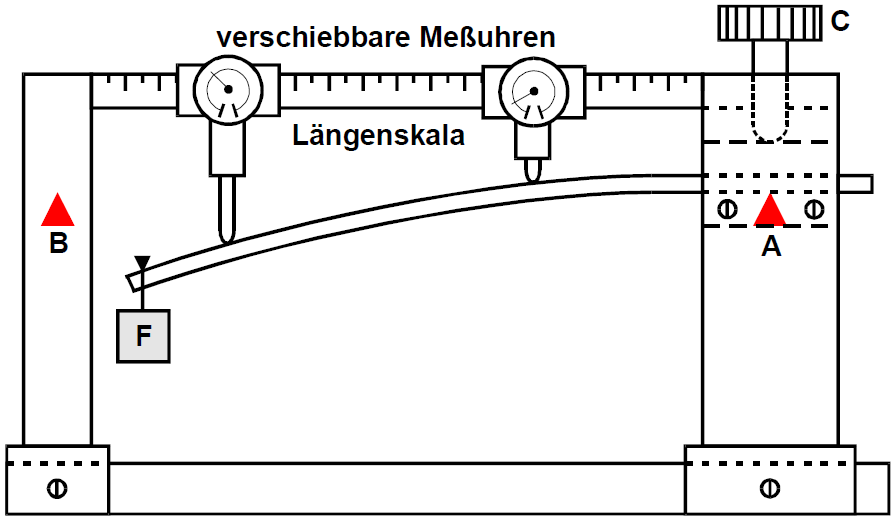
\includegraphics[height=6cm]{data/bild_3}
    \caption{Aufbau für Einseitige Einspannung}
    \label{fig:aufbau1}
\end{figure}

Wie in Abb.\ref{fig:aufbau1} wird eine Metallstange an einer Seite des Gestells eingespannt. Von der Abbildung abweichend ist hier nur eine Messuhr
verbaut. Dieser Aufbau wird mit zwei unterschiedlichen Metallstangen durchgeführt. Für beide wird jeweils eine Messung ohne angehängtes
Gewicht als Abgleich durchgeführt. Danach wird ein Gewicht von  $m_1 = 1.2096 \si{\kilo\gram}$ an das lose Ende der Metallstange angebracht und 
der Versuch wird nocheinmal durchgeführt. Dabei wird die Messuhr, am festen Ende beginnend, in 3$\si{\centi\meter}$ Schritten entlang der 
Stange verschoben. Bei jedem Schritt wird die Auslenkung der Stange über die Messuhr abgelesen. Es ist dabei wichtig, darauf zu achten,
dass die jeweilige Stange zwischen Nullmessung und Messung mit Gewicht nicht verdreht wird, da nicht davon ausgegangen werden kann, dass 
die Stange perfekt gerade ist. Daher würde das Messergebnis bei einer Verdrehung verfälscht werden. 

\subsection{Beidseitige Auflage}

Bei dieser Variante wird die Metallstange, wie in der abb[] zu sehen ist, an zwei Punkten aufgelegt, aber nicht eingespannt. Daher muss 
hier besonders darauf geachtet werden, dass die Stange weder verschoben, noch verdreht wird. Es wird, wie im vorherigen Versuch, für 
beide Stangen jeweils eine Nullmessung, also ohne angehängtes Gewicht, und eine Messung mit angehängtem Gewicht durchgeführt. Bei beidseitiger Auflage muss ein schwereres Gewicht angebracht werden, da es sonst kaum zu eine Durchbiegung kommt. Hier wird ein Gewicht von $m_2 = 4.7166 \si{\kilo\gram}$ verwendet.
Das Gewicht wird hierzu in der Mitte der beiden Auflagepunkte angebracht. Dann werden zwei Messuhren zueinander symmetrisch um das 
angehängte Gewicht verwendet, um die Auslenkung der Stange zu messen. Die Messungen werden in 1$\si{\centi\meter}$ Schritten, im Zentrum 
der Stange beginnend, vorgenommen. 